\documentclass[a4paper,12pt,numbers=noenddot]{report}

\usepackage{polski}
\usepackage[utf8]{inputenc}
\usepackage{graphicx}
\usepackage{cite}
\usepackage{float}
\usepackage{url} 
\usepackage{hyperref}
\usepackage{amsmath}
\usepackage{gensymb}
\usepackage{pdfpages}
\usepackage[nottoc,numbib]{tocbibind}
\usepackage{etoolbox}
\usepackage{enumitem}

\usepackage{titlesec, blindtext, color}

\titleformat{\chapter}[hang]{\Huge\bfseries}{\thechapter{. }}{0pt}{\Huge\bfseries}


\usepackage[
  inner = 3cm,
  outer = 2.5cm,
  top = 2.5cm,
  bottom = 2.5cm,
]{geometry}


\title{TYTUŁ pracy}
\date{\today}
\author{Hubert Marcinkowski}

\begin{document}
	\nocite{*}
	\pagenumbering{gobble}
	\maketitle
	%\includepdf{title2.pdf}

	\newpage
	\pagenumbering{arabic}
	\tableofcontents
	\newpage
	%\setcitestyle{square}	
	
\chapter{Wstęp}
Projektowanie interfejsów jest tematyką bardzo złożoną i nadzwyczaj kluczową w procesie tworzenia aplikacji, w tym, między innymi, gier komputerowych. Złe zaprojektowanie tej części w prosty sposób może przyczynić się do całkowitego braku zrozumienia całego przesłania gry przez użytkowników. Istnieje wiele metodologii mających na celu analizę jakości stworzonego projektu - od metod całkowicie subiektywnych po takie, które stawiają za zadanie sprowadzenie jak największej części elementów do postaci parametrycznej. 

- Trudne zadanie związane z tym, że poszukiwany jest pewien zbiór reguł, który ułatwiłby proces projektowania. 
- Część z przedstawianych rozwiązań wybitnie nie pasuje do dziedziny mobilek
- Problemy związane z projektowaniem dla mobilek
- Przygotowane zostały heurystyki, które mają na celu dokładne określenie jakie warunki aplikacja musi spełniać, by mogła zostać dobrze odebrana przez użytkowników
- coś o tym, że użytkownik w czasie gry często zostaje postawiony przed przyswojeniem bardzo abstrakcyjnego zadania w celu zrozumienia, a co za tym idzie grania w daną grę

W pracy tej opisane zostało badanie mające na celu zweryfikowanie wpływ spełniania tych heurystyk na pozna

\chapter{Cel, założenia oraz zakres pracy}
Celem tej pracy było zbadanie wpływu określonych heurystyk tworzenia interfejsów na jakość przyswajania nowych mechanik gry mobilnej. Zbadane zostały wybrane dwie opisane przez H. Desuvire oraz Ch. Wiberg [odnośnik!] reguły, które odnoszą się do użyteczności projektowanych aplikacji.

!
Zwykle heurystyki dla gier mobilnych sprawdzają grywalność, tutaj wykorzystane zostają, by sprawdzić ich wpływ na jakość przyswojenia nowych reguł przedstawianych użytkownikowi, mechanik rozgrywki.
!

Przeprowadzone zostało doświadczenie, które miało na celu określenie, czy gra, której interfejs spełnia zadane warunki jest lepiej rozumiana i szybciej opanowywana od takiej, której nie są spełnione wybrane heurystyki. Przygotowana została w tym celu aplikacja na urządzenia mobilne, w której użytkownikom postawione zostają zadania, które nie wpisują się w popularne szablony obecnych gier na te platformy. Wyróżnione zostały cztery różne wersje interfejsów przedstawianych użytkownikowi, każda wersja spełniała inny złożenie heurystyk.

\chapter{Wyjaśnienie pojęć}
Grywalność - 

Kontrola -

\chapter{Analiza podobnych rozwiązań}

Tutaj opisuję inne rozwiązania? badania?

\chapter{Gra mobilna}
\textit{Sphaze} - gra, która wykorzystana została na potrzeby badań należy do gatunku gier logicznych. Przed użytkownikiem postawione jest abstrakcyjne zadanie doprowadzenia obracających się kul do środka labiryntu składającego się z współcentrycznych pierścieni. Sfery poruszają się jedynie po wyraźnie zarysowanych ścieżkach. Wygląd przykładowego poziomu zawierającego dwie kule oraz trzy pierścienie zamieszczony został na rysunku \ref{fig:sphaze_1}.

\begin{figure}[h!]
	\centering
  	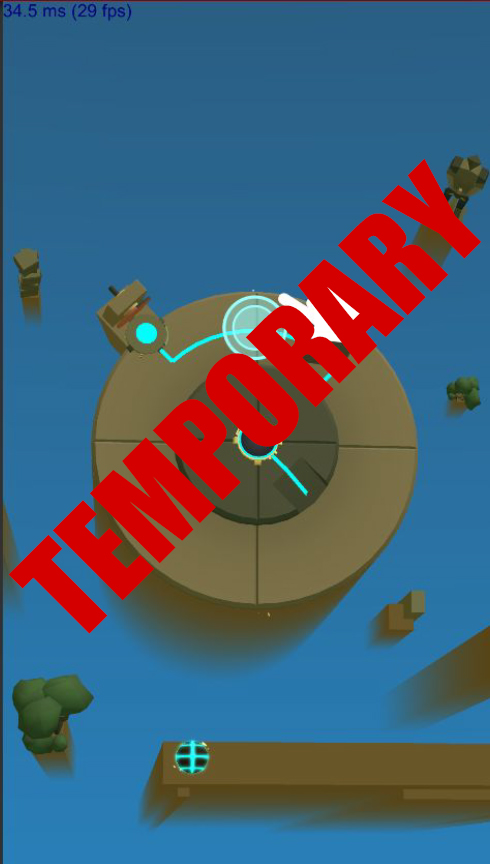
\includegraphics[height=10cm]{fig/tmp.jpg}
	\caption{Wygląd przykładowego poziomu gry \textit{Sphaze}.}
	\label{fig:sphaze_1}
\end{figure}

Osoba grająca nie ma wpływu na ruch sfer, jedynie na obrót pierścieni planszy. Każda rotacja na tych elementach powoduje zmianę połączeń między ścieżkami na nich się znajdującymi. Kule cały czas poruszają się do przodu, chyba że spotkają na swojej drodze skrzyżowanie. Wybierają wtedy ścieżkę, którą zdefiniować można jako "najbardziej prawą". Oznacza to, mając możliwość skręcenia w prawo, zawsze wybiorą tą opcję. Gdy nie ma możliwości obrotu w prawo, sprawdzane jest, czy dostępna jest ścieżka na wprost. W następnej kolejności przeprowadzony zostaje test, czy istnieje skręt w lewo. W przypadku braku możliwości wyboru żadnej z przedstawionych opcji, uznawane jest, że natrafiono na "ślepy zaułek", konieczne jest zatem zawrócenie.

Użytkownik decyduje również, z którego miejsca na planszy ma wystartować jaka sfera. Wprowadzenie pierwszej kuli na strefę labiryntu traktowane jest jako rozpoczęcie rozgrywki. Przykładowe punkty startowe, na których ustawić można kule ukazane zostały na rysunku \ref{fig:sphaze_startpoints_1}. Zauważyć można, iż znajdują się one wszystkie na obrzeżach planszy. Jest to reguła, którą gracz jest w stanie bardzo szybko zauważyć. Dzięki temu na późniejszych poziomach gracze nie próbują ich szukać w żadnym innym miejscu. Z racji na fakt, iż "rozbijają" one okrągłą sylwetkę planszy wyjątkowo łatwo je dostrzec nawet gdy gra aktualnie ich nie wyróżnia. 
Na każdym poziomie zdefiniowane jest ograniczenie czasowe, którego przekroczenie jednoznacznie wiąże się z koniecznością powtórzenia zadanej planszy. Czasomierz, którego zadaniem jest informowanie użytkownika o tym jak dobrze sobie on radzi, rozpoczyna odliczanie wraz z rozpoczęciem rozgrywki, czyli gdy pierwsza kula zacznie poruszać się w przestrzeni poziomu. 

\begin{figure}[h!]
	\centering
  	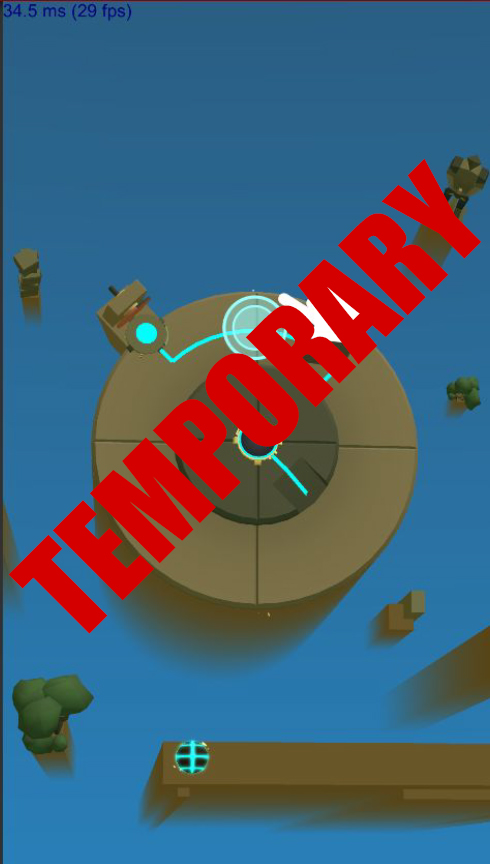
\includegraphics[height=10cm]{fig/tmp.jpg}
	\caption{Przykładowe rozmieszczenie punktów startowych na poziomie. Punkty startowe zostały oznaczone czerwonymi okręgami.}
	\label{fig:sphaze_startpoints_1}
\end{figure}

Gracz ma ograniczoną kontrolę nad rozgrywką, gdyż jego akcje wpływają jedynie pośrednio na jej przebieg. Obrót pierścieni wpływa jednie na możliwości ruchu, jakimi dysponują kule. Zadaniem użytkownika jest dostosowanie się do tego stanu i przewidzenie, jak obiekty poruszać się będą w zadanym przez niego środowisku. Nieświadome podejmowanie decyzji może bowiem prowadzić do sytuacji, które szybko potrafią stać się mało zrozumiałe dla użytkownika, który nie do końca rozumie, co się dzieje w przestrzeni gry.

	\subsection{Samouczki}
Wymagane jest zatem, by gracz przyswoił podstawowe prawa tej gry jak najszybciej. W przeciwnym wypadku spodziewać się można, iż prędko zacznie odczuwać frustrację spowodowaną pozornie małym wpływem jego akcji na finalny wynik gry. 

Z tego też powodu przygotowane zostały tzw. samouczki mające na celu wyjaśnienie użytkownikowi kluczowych mechanik. Nowe informacje przekazywane są stopniowo. Każdy kolejny element kluczowy jest najpierw przedstawiany w prostym, kontrolowanym środowisku, a następnie powtarzany już w coraz bardziej złożonych sytuacjach. 
W przeprowadzanym badaniu analizowane były trzy główne mechaniki: 
\begin{itemize}
\item sposób na startowanie rozgrywki na danym poziomie, 
\item obracanie pierścieniami,
\item ruch kulek (fakt, iż zawsze skręcają one w najbardziej prawą ścieżkę.
\end{itemize}

W celu poprawnego nauczenia tych mechanik przygotowane zostały dwa testowe poziomy. W pierwszym z nich przedstawiane są podstawowe dwie zasady gry. Akcja jaką, użytkownik ma wykonać zostaje przedstawiona wizualnie bez użycia tekstu. Sam gracz musi zrozumieć, że jego ruchem powinno być odzwierciedlenie tego, co pokazywane mu jest na ekranie. Należy zauważyć, że użytkownik nie zawsze jest w stanie również przewidzieć co się wydarzy, gdy wykona zadane mu zadanie. Dopiero po wykonaniu ukazanej akcji jest w stanie przeanalizować jaki wpływ miały jego ruchy na przestrzeń gry.
Wygląd poszczególnych etapów tego poziomu dla jednej wersji gry przedstawiony został na rysunku \ref{fig:tut_L1_1}.

\begin{figure}[h!]
	\centering
  	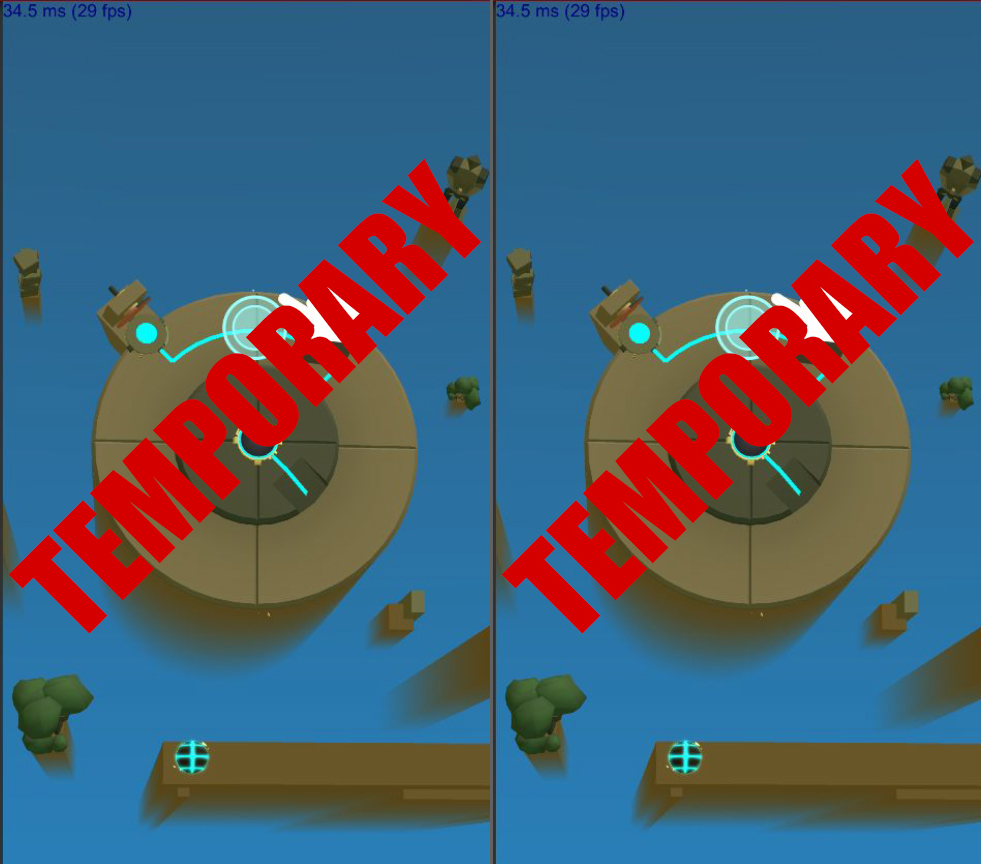
\includegraphics[height=10cm]{fig/tmp2.jpg}
	\caption{Wygląd pierwszego samouczka przed którym postawiony jest gracz.}
	\label{fig:tut_L1_1}
\end{figure}

Plansza dla tego poziomu składa się z dwóch poziomu składa się z dwóch pierścieni. Nie można poruszać pierścieniem w samym środku, co sprawia, że jedynym fragmentem labiryntu, z którym użytkownik może wchodzić w interakcję jest zewnętrzny pierścień.
Gdy gracz włączy ten poziom wymagane jest od niego aby najpierw obrócił właśnie ten element. Celem jest doprowadzenie do połączenia ścieżek znajdujących się na pierścieniach. Gdy gracz wykona ruch powodujący rozłączenie tych dróg, samouczek powróci do tego etapu. Pozwala to w łatwy sposób uzmysłowić użytkownikowi, o wadze, jaką ma stworzenie odpowiedniej drogi dla kul. 
Następnym zadaniem jest ustawienie jedynej sfery na poziomie w jej miejscu startowym. Samouczek znika dopiero w momencie poprawnego wykonania tej akcji. Gdy to nastąpi i użytkownik nie wprowadzi dalszych zmian w obrocie pierścieni, kula w szybki sposób dociera do środka labiryntu, a co za tym idzie - kończy poziom.

Drugi samouczek ustawiony został dopiero na trzeciej planszy. W tym miejscu chcemy zwrócić uwagę gracza na zachowanie kul w momencie dotarcia do skrzyżowania. Wygląd tego poziomu zobaczyć można na rysunku \ref{fig:tut_L3_1}. Labirynt w tym wypadku składa się z trzech pierścieni, z czego z dwoma z nich użytkownik może wejść w interakcję. Obecny tutaj samouczek wyzwala się dopiero w momencie, gdy za przeprowadzonymi wcześniej akcjami gracza sfera dotrze do skrzyżowania znajdującego się na środkowym pierścieniu. Zostaje wtedy zabrana użytkownikowi kontrola a kamera skupia się na problematycznym miejscu. Oprócz tego, zanim zostanie wykonany manewr kulki, zostaje pod nią narysowana strzałka wskazująca, w którą stronę ona skręci. Całość opisanych akcji zajmuje podczas normalnej gry tylko ułamek sekundy, dlatego czas gry zostaje w tym momencie czterokrotnie spowolniony. Gry kulka opuszcza skrzyżowanie, kamera wraca do podstawowej pozycji a ruchy gracza znowu wpływają na układ pierścieni. 

\begin{figure}[h!]
	\centering
  	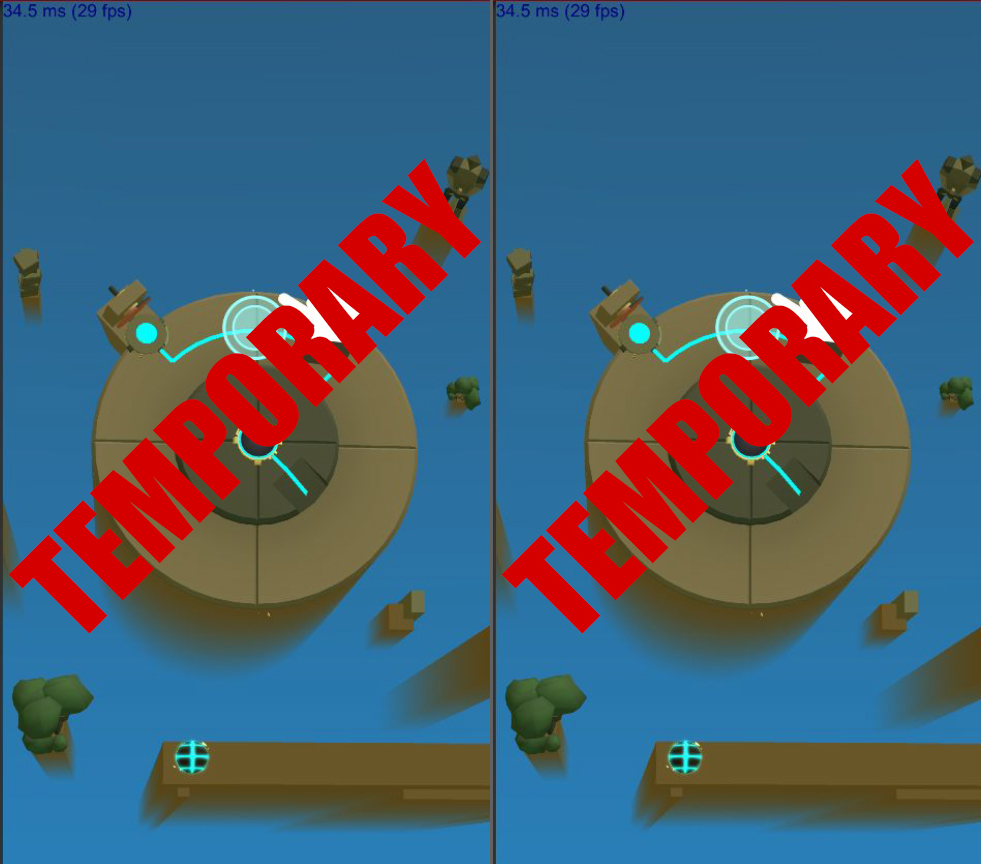
\includegraphics[height=10cm]{fig/tmp2.jpg}
	\caption{Wygląd poziomu zawierającego samouczek tyczący się skrętu kul. Czerwonym okręgiem zaznaczone zostało skrzyżowanie.}
	\label{fig:tut_L3_1}
\end{figure}


\chapter{Metoda badawcza}
	\section{Hipotezy}
Hipoteza 1.

Hipoteza 2.
	\section{Badanie}
Pierwsza hipoteza
Druga hipoteza

\chapter{Wyniki badań}
Tu przedstawiam wyniki badań
\chapter{Wnioski}
Poziom 3 zabiera kontrolę i to się graczom nie podobało. Układ poziomu wpływa na to, że gracze szukają tam "podstępu".

\chapter{Zakończenie}
Tu podsumuję?

%\pagenumbering{gobble}

\chapter{Zawartość płyty}
\begin{enumerate}[label={[\arabic*]}]
  \item Tekst pracy w formacie PDF
  \item Pliki z wynikami przeprowadzonych badań
  \item Plik z wynikami przeprowadzonej analizy
\end{enumerate}

%TODO: Bibliografia
\end{document}
